\documentclass[12pt,a4paper]{scrartcl}
\usepackage[protrusion=true,expansion=true]{microtype}
\linespread{1.25}

\usepackage{float}
\usepackage{amssymb}
\usepackage[utf8]{inputenc}
\usepackage[T1]{fontenc}
\usepackage{graphicx}
\usepackage[bookmarks=true,hidelinks=true,breaklinks=true]{hyperref}
\usepackage{mathptmx}
\usepackage{cleveref}
\usepackage{enumitem}
\usepackage[backend=biber,natbib=true]{biblatex}
\usepackage[scaled=.92]{helvet}
\bibliography{references.bib}

\newtheorem{lemma1}{Lemma}

\begin{document}
\title{Der Transparente Mensch: Die unvermeidliche Preisgabe von Metadaten }
\author{Arne Beer, MN 6489196, University of Hamburg}
\date{20.08.2019}

\maketitle


\section{Abstract}

Metadaten spielen eine bedeutende Rolle in der Welt der Datenanalyse.
Simple Informationen über einen Menschen, wie zum Beispiel der Standort verknüpft mit Zeitpunkten, verschiedene Aktivitäten oder Vorlieben, liefern enormes Potential, um diesen zu analysieren und kategorisieren.
In vielen Fällen wird aktives Sammeln von Daten, Data Mining und Big Data Analysis betrieben und Plattformen wie Facebook, haben sich voll diesem Ziel verschrieben.

Metadaten sind jedoch tückisch und befinden sich an viel mehr Orten als man vielleicht auf den ersten Blick vermutet.
Dieses Paper wird sich speziell mit der Intransparenz in Bezug auf die Freigabe von Metadaten bei bestimmten Tools auseinandersetzen, welche eigentlich nicht für diesen Zweck vorgesehen sind.
Speziell betrachten wir in diesem Falle das Tool \emph{Git}, welches hauptsächlich zur Versionskontrolle von Quellcode in Informationstechnischen Projekten verwendet wird.
Zudem wird die populäre Website \emph{GitHub} betrachtet, welche als Open-Source Plattform dient, auf der jeder Entwickler seine Projekte öffentlich zur Verfügung stellen kann.

\section{Einleitung}

\section{Git und GitHub}

\section{Literatur}

\section{Probabilistic Simhash Matching}

%\begin{figure}[H]
%    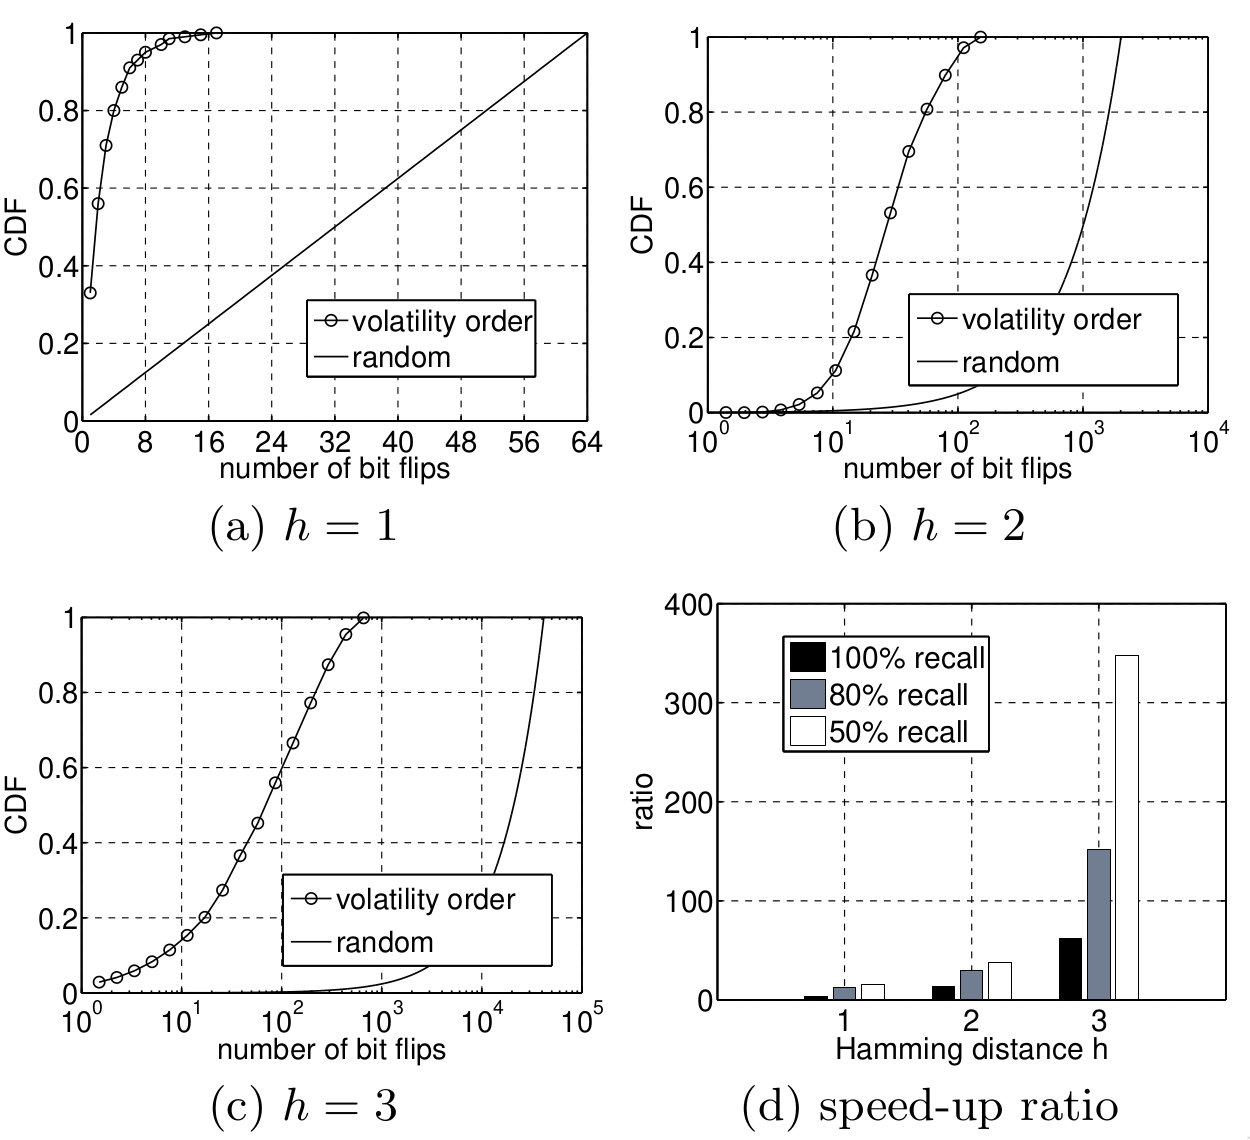
\includegraphics[scale=0.33]{./gfx/vosh-performance.png}
%    \centering
%    \caption{Performance results comparing random comparison search and volatility order based search.}\label{fig:vosh-performance}
%\end{figure}


\section{Zusammenfassung}

\printbibliography
\end{document}
